\section{Geometry Editor}

This article is designed to outline the basic controls of ICE's Geometry Editor.

\subsection{Getting Started}

Once ICE is installed on your computer, there are no further dependencies or
preparation required to use the Geometry Editor.

\subsection{Opening a Geometry Editor}

To open a Geometry Editor in ICE, you have three options:

\begin{center}
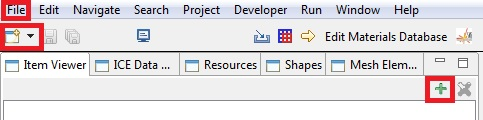
\includegraphics[width=12cm]{images/CreateNewGeometryOptions.jpg}
\end{center}

Top to bottom, they are:

1) Click the File menu, then New, then Other\ldots and select the Create Item
Wizard in the new dialog and press Next. Then, select Geometry Editor from the
list and press Finish.

 
2) Click the New button. Select Create Item Wizard in the new dialog and
press Next. Then, select Geometry Editor from the list and press Finish.


3) Enter the ICE Perspective by clicking the Open Perspective button in the
upper right corner of the screen, select ICE from the dialog that pops up, and
click OK. Afterwards, click the Create an Item button, select Geometry Editor,
and click OK.

\subsection{Working with the Geometry Editor}

\subsubsection{Camera}

You can change the perspective of the camera by clicking and dragging inside the
Geometry Editor. You can see this initially by the way the three axes and the
reference plane move as you rotate the camera about the origin. If you hold
shift while dragging, you will instead move the central point the camera is
focused on. If you hold ctrl, you can drag the mouse up or down to zoom in or
out, respectively. Scrolling the mouse wheel offers another way to zoom the camera.

\subsubsection{Primitive Shapes}

\begin{center}
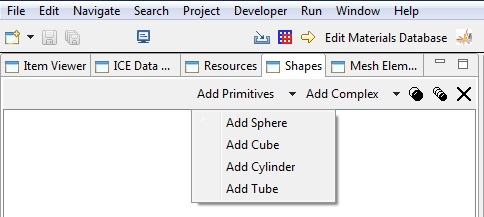
\includegraphics[width=12cm]{images/GeometryAddPrimitive.jpg}
\end{center}

Simple shapes can be added with the Add Primitives dropdown menu in the Shapes
view. Simply select an object from the menu to add it to the scene.

\begin{center}
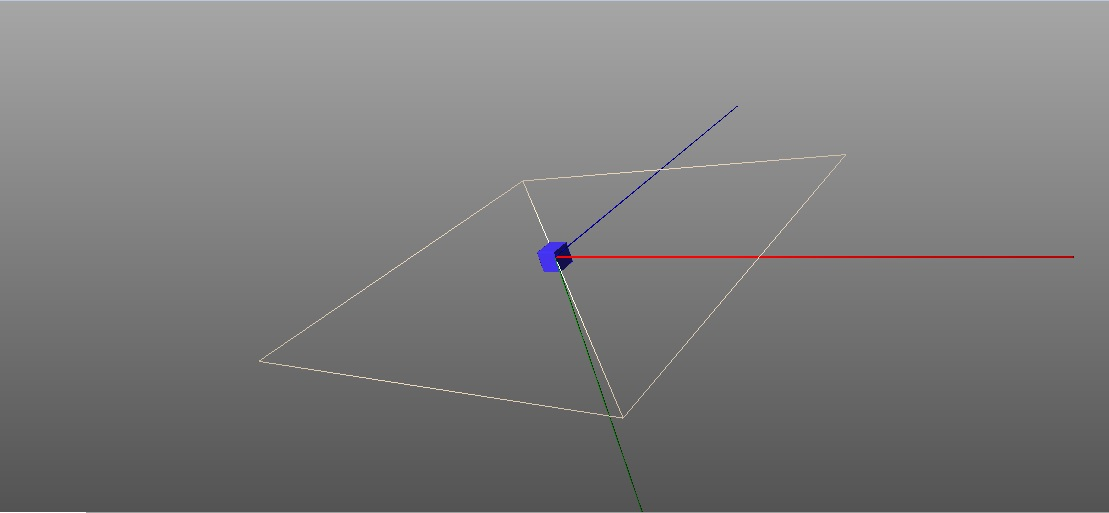
\includegraphics[width=12cm]{images/GeometryAddCube.jpg}
\end{center}

Clicking on the shape's name in the Shapes View will cause that shape and any
children to appear in the Properties view. 

\begin{center}
\includegraphics[width=12cm]{images/GeometryPropertiesView.jpg}
\end{center}

Editing the values in this view will change the selected shape
accordingly. 

\begin{center}
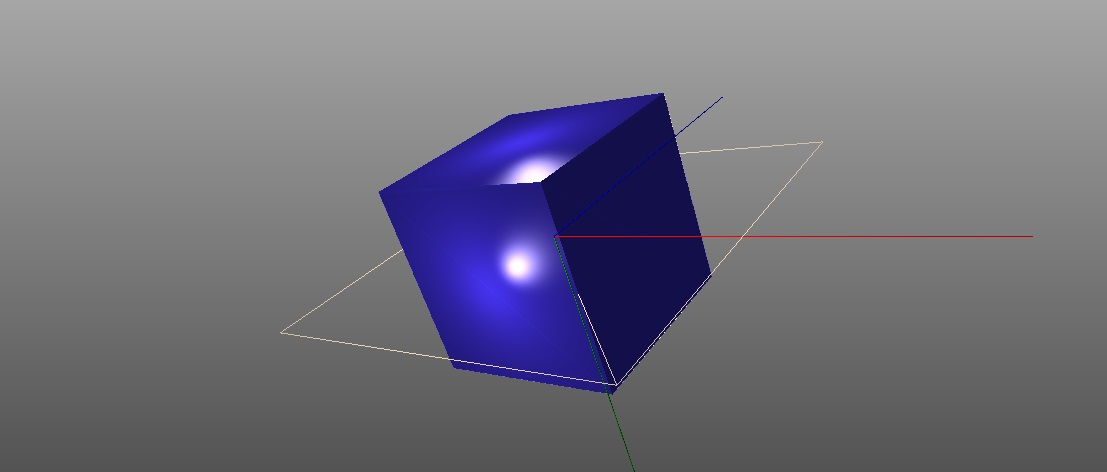
\includegraphics[width=12cm]{images/GeometryCubeSize.jpg}
\end{center}

\textbf{Mesh Properties} - These controls will allow the user to set any custom
properties of the mesh. A cube has ``sideLength'', which will control the size
of the cube.

\begin{center}
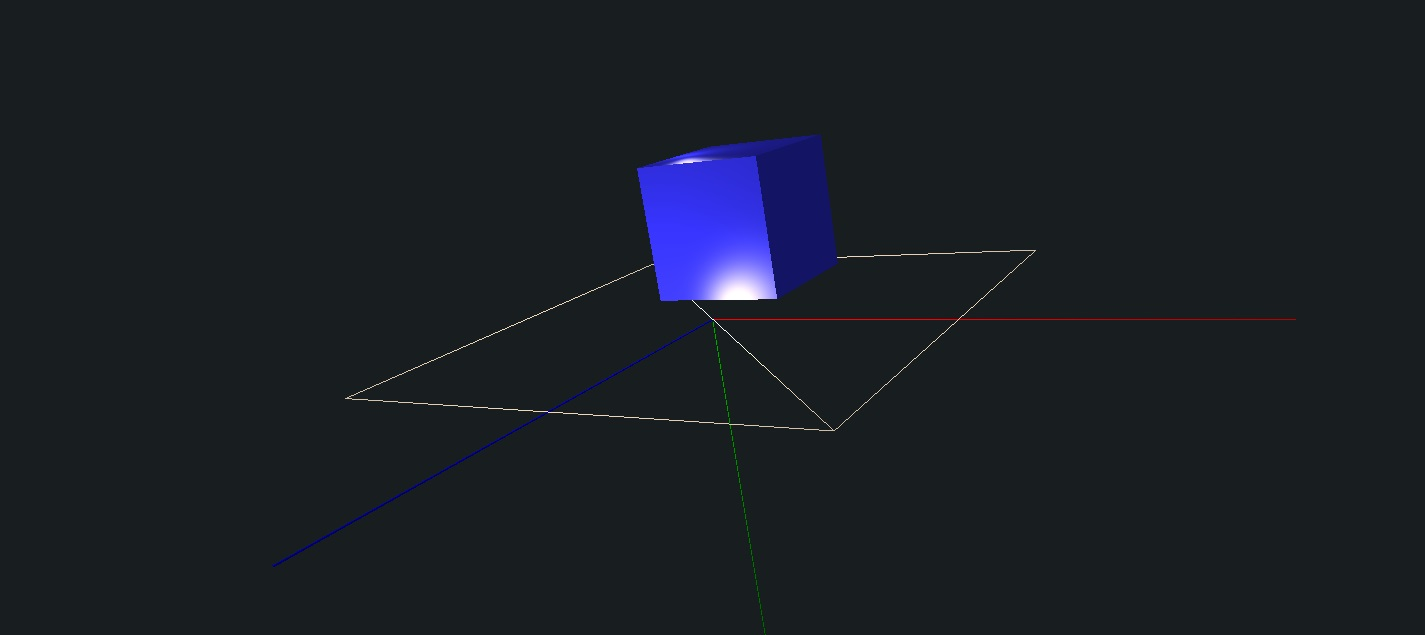
\includegraphics[width=12cm]{images/GeometryCubeTranslate.jpg}
\end{center}

\textbf{Center} - These controls allow the shape to be moved about hte three
dimensional space by setting the X, Y, and Z coordinates of its center.

\textbf{Triangle Mesh Data} - This table list the coordinates for all vertices
in each triangle used to define the shape.

\begin{center}
\includegraphics[width=12cm]{images/GeometryCubeColor.jpg}
\end{center}

\textbf{Color} - These controls allow for setting the shape's color.

\begin{center}
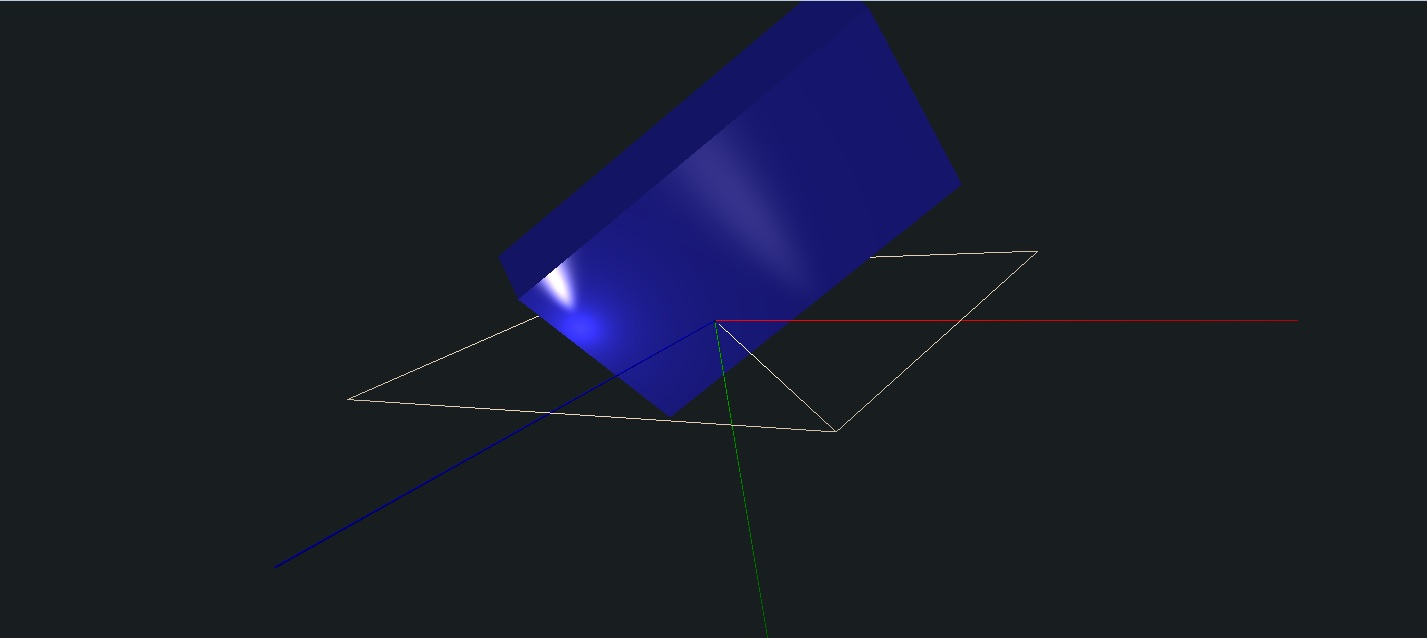
\includegraphics[width=12cm]{images/GeometryCubeScale.jpg}
\end{center}

\textbf{Scale} - Controls the magnification of the shape. For more complex
shapes such as tubes or imported files, it is a simpler way to set the
geometry's size.

\begin{center}
\includegraphics[width=12cm]{images/GeometryCubeWireframe.jpg}
\end{center}

\textbf{Opacity} - This menu allows for a shape to be displayed as a wireframe
or to be rendered transparent and removed from the scene.

\begin{center}
\includegraphics[width=12cm]{images/GeometryCubeDisplayDeactivated.jpg}
\end{center}

The check boxes by each display option allow that effect to be toggled, allowing
you to quickly change a shape back and forth from its default display to your
custom settings. Notice how the cube remained the same size, as it was edited to
be larger, while the tube was kept the same size but had only been set to draw
larger in the display menu.

\subsubsection{Complex Shapes}

Multiple primitive shapes can be combined within a single grouping for easier
editing. First, create a complex shape using the Add Complex button. 

\begin{center}
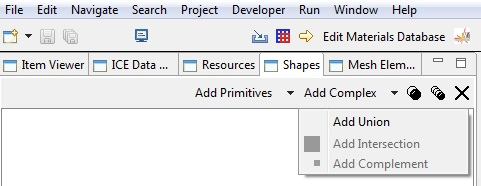
\includegraphics[width=12cm]{images/GeometryAddComplex.jpg}
\end{center}

Currently, only unions are supported. The union will appear in the Shapes View
with an empty spot for a child shape. 

\begin{center}
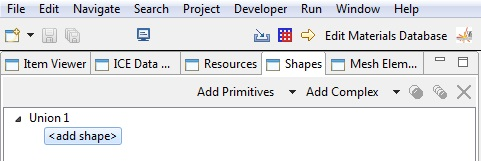
\includegraphics[width=12cm]{images/GeometryUnionAddShape.jpg}
\end{center}

Select \textless Add Shape\textgreater and add a primitive shape as before to
add the shape as a child of the union. To add additional shapes, select the
child shape and add another as normal.

Selecting the union will select all of its child shapes, and changes to the
Properties View will affect the entire complex shape. Individual shapes can
still be selected for editing on their own, but you must deactivate all parent
shape's display options if they conflict with the childrens.

\begin{center}
\includegraphics[width=12cm]{images/GeometrySlotMachineMonochrome.jpg}
\end{center}

For example, this slot machine is a union of shapes. While the union is set to a
purple color, all child shapes are also set to purple. 

\begin{center}
\includegraphics[width=12cm]{images/GeometrySlotMachineMonochrome.jpg}
\end{center}

By deactivating the union's color display, the child shapes will each be able to
display their own color.

\begin{center}
\includegraphics[width=12cm]{images/GeometrySlotMachineColor.jpg}
\end{center}

You can add a complex shape as a child to a complex shape in the same way as a
primitive shape, allowing for nested unions

\subsubsection{Copying}

Once you have a shape created, you can automatically create copies of that
shape. 

\begin{center}
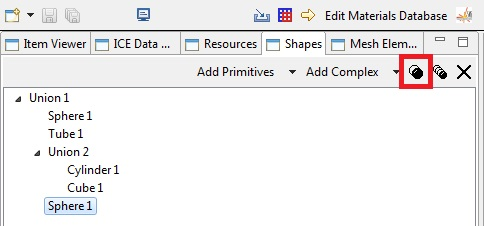
\includegraphics[width=12cm]{images/GeometryDuplicateShape.jpg}
\end{center}

Press the Duplicate Shape button, highlighted above, to create an exact copy of
the selected primitive shape. The copy will appear as the child of the same
complex shape as the original, if any, and can be modified independently after
creation.

\begin{center}
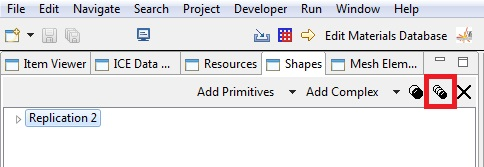
\includegraphics[width=12cm]{images/GeometryReplicateShape.jpg}
\end{center}

You can systematically create many copies of a shape with the Replicate Shape
button highlighted above. This will open a new dialog.

\begin{center}
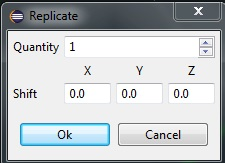
\includegraphics[width=8cm]{images/GeometryReplicateDialog.jpg}
\end{center}

The quantity is the number of desired copies of the shape which should be in the
replication. This includes the original (ie setting quantity to 2 will result in
2 shapes, the original and a copy).

The Shift boxes allow you to specify an offset to be placed between each copy.
For example, if you set X to 100 and Y to 50, then each copy will be 100 units
along the X axis and 50 along the Y away from the previous copy. 

The original shape and all copies will be placed in a new complex shape, which
will take the original shape's position in the tree.

\subsubsection{Deletion}

You may remove a shape and all its children by selecting it in the Shapes view
and clicking the Delete button, highlighted below.

\begin{center}
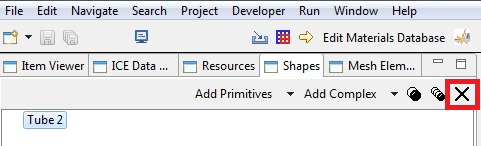
\includegraphics[width=12cm]{images/GeometryDeleteButton.jpg}
\end{center}

\subsubsection{Importing}

The Import File button next to Add Primitive will add import the contents of an
.obj or .stl file. These will appear as a union containing other shapes inside. 

\subsubsection{Saving}

You may save the contents of the Geometry Editor. This can be done as normal for
an Eclipse file, using the Save button or \texttt{Ctrl + S}. The result will be
a file named Geometry\_Editor.xml in the ItemDB folder. The Geometry Editor can be
reponed by double clicking on this file. 
